% IEEE Paper Template for US-LETTER Page Size (V1)
% Sample Conference Paper using IEEE LaTeX style file for US-LETTER pagesize.
% Copyright (C) 2006-2008 Causal Productions Pty Ltd.
% Permission is granted to distribute and revise this file provided that
% this header remains intact.
%
% REVISION HISTORY
% 20080211 changed some space characters in the title-author block
%
\documentclass[10pt,conference,letterpaper]{IEEEtran}
\usepackage{times,amsmath}
\usepackage{multirow}
\usepackage{graphicx}
\graphicspath{ {images/} }
%
\title{Cohana Demo}
%
%\author{%
% author names are typeset in 11pt, which is the default size in the author block
%{First Author{\small $~^{\#1}$}, Second Author{\small $~^{*2}$}, Third Author{\small $~^{\#3}$} }%
% add some space between author names and affils
%\vspace{1.6mm}\\
%\fontsize{10}{10}\selectfont\itshape
% 20080211 CAUSAL PRODUCTIONS
% separate superscript on following line from affiliation using narrow space
%$^{\#}$\,First-Third Department, First-Third University\\
%Address Including Country Name\\
%\fontsize{9}{9}\selectfont\ttfamily\upshape
%
% 20080211 CAUSAL PRODUCTIONS
% in the following email addresses, separate the superscript from the email address 
% using a narrow space \,
% the reason is that Acrobat Reader has an option to auto-detect urls and email
% addresses, and make them 'hot'.  Without a narrow space, the superscript is included
% in the email address and corrupts it.
% Also, removed ~ from pre-superscript since it does not seem to serve any purpose
%$^{1}$\,first.author@first-third.edu\\
%$^{3}$\,third.author@first-third.edu%
% add some space between email and affil
%\vspace{1.2mm}\\
%\fontsize{10}{10}\selectfont\rmfamily\itshape
% 20080211 CAUSAL PRODUCTIONS
% separated superscript on following line from affiliation using narrow space \,
%$^{*}$\,Second Company\\
%Address Including Country Name\\
%\fontsize{9}{9}\selectfont\ttfamily\upshape
% 20080211 CAUSAL PRODUCTIONS
% removed ~ from pre-superscript since it does not seem to serve any purpose
%$^{2}$\,second.author@second.com
%}
%
\begin{document}
\maketitle
%
\begin{abstract} 
The tremendous volume of user behavior activities records generated in various domains provides data analysts an opportunity to mine insights towards the users. Cohort analysis, aiming to find user behavioral trends in large tables, is one of the most commonly used techniques. Regarding the fact that cohort analysis suffers from the traditional database systems in both operability and efficiency, we proposed a cohort query engine, i.e., Cohana. Taking advantage of the overwhelming performance of Cohana, we further present a comprehensive and powerful tool covering a majority of needs in cohort analysis, all the while requires intuitive and accessible operations. We demonstrate analytics can easily define their requirements, and conduct the analysis or verify their assumptions on user behavior with our system in no time.
\end{abstract}

% NOTE keywords are not used for conference papers so do not populate them
% \begin{keywords}
% keyword-1, keyword-2, keyword-3
% \end{keywords}
%
\section{Introduction}
%
In an era where most user activities are electronically recorded either actively or passively, people reach the consensus that we can gain insights towards user behavior from that accumulated huge amount of data, which further brings both commercial and public interests. With the maturity of data storage and cleansing techniques, we are more keen on analyzing and explaining the complete data.

The need of data analysis on the user activities records throws out challenges on plain analytics techniques such as SQL GROUP BY, and thus emerged Cohort analysis. In fact, there are two decisive factors affecting human behavior [9]: aging and social changes, i.e., people change their behavior when they grow older, as well as the societies they live in evolve, precisely the conditions Cohort analysis focuses on while assessing. The Cohort analysis studies the human behavioral by determining: 1) the groups users belong to; 2) the births and ages of user activities; 3) aggregation methods in each group and age. With the three definitions, Cohort analysis provides abstract and complete descriptions on user behavior study. The following example is a standard issue in the medical area. Though apparently troublesome for SQL GROUP BY, it can be easily handled by Cohort analysis as long as the three definitions are settled.

\emph{\textbf{Example:} A hospital wants to know the side effects of a new medicine A on patients divided by different ages who are diagnosed with disease B. The monitoring on the effects begins after a patient taking the medicine at least 2 times, and is indicated by abnormal values in daily-conducted lab-test C.}

However, it is both painful to specify and expensive to evaluate for cohort analysis in traditional database systems. Therefore, we designed the new cohort operators and proposed Cohaha[ref], an efficient cohort query processing engine. The cohort query is more concise and accurate than SQL query, and the specially designed storage manager and query executor in Cohona brings overwhelming performance superiority against traditional database systems. 

Further, we develop a web interface on the top of Cohana to provide users intuitive and powerful cohort query services. Users determine the cohort analysis conditions by selecting options described in natural language interactively on the web page instead of writing cohort queries, which is acceptable for those without query knowledge. What's more, owing to the efficiency of the backend Cohana engine, the results of queries are displayed and visualized on the web page in no time. In one word, users can insight the data swiftly, accurately, and intuitively. 

In this demo, we will walk through...

Contribution
\begin{itemize}
\item	C1
\item   C2
\item   C3
\end{itemize}

\section{System Overview}
In this section, we briefly introduce the three key definitions in cohort query firstly, and then depict the overall system architecture, including the data pre-processing, the front-end web interface, and the back-end Cohana engine, to explain the whole process of a Cohort analysis.  

\subsection{Query Definition}
As discussed in the previous section, a typical Cohort analysis requires defining \textbf{cohort}, \textbf{birth and age}, and \textbf{aggregation}. 

\textbf{Cohort -} Cohort refers to a group of users sharing some common characteristic. Users are separated into different cohorts according to the features they have when performing a given action for the first time. For example, we can cohort patients by the disease diagnosed when initially admitted to the hospital. Notice that the characteristics may change over time, and we cohort on the basis of features by the time of particular action.

\textbf{Birth and age -} A user \emph{i} is considered born when firstly performing a specific birth event \emph{e}, and the birth time is exactly the time of that event, or -1 if \emph{i} never made \emph{e}. The age \emph{g} is to specify the time slice for aggregation since birth time. For example, if we define the birth event as taking lab test and age as one day, a patient firstly recorded the lab test on January 1st will be at age 1 on January 2nd. Another patient firstly taking the test on March 4th will also be at age 1 on March 5th, regardless of different birth time.

\textbf{Aggregation -} Aggregation refers to the calculation function conducted on the user activity records within same cohort and age. Users can perform aggregation as simple as counting the occurrence, or as complex as fitting distribution. For example, we can check the retention rate of patients by counting off patients' admission records every month (i.e., age) after being discharged (i.e., birth event).

\subsection{System Architecture}

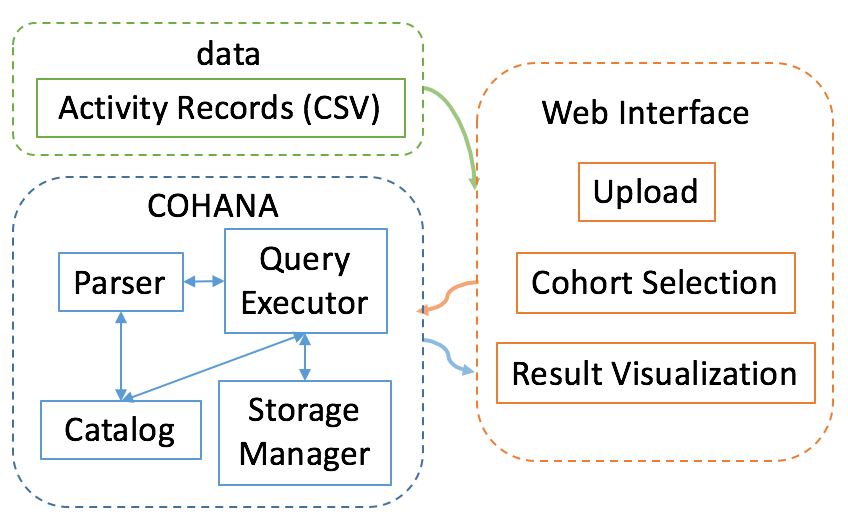
\includegraphics[width=0.4\textwidth]{arch.png}

Figure 1 outlines the architecture including three components, i.e., data, Cohana engine and web interface, and data flow among the components.

\begin{center}
\begin{tabular}{ |c|c|c|c| }
\hline
Item & Options & Description \\
\hline
name & & unique values \\
\hline
\multirow{5}{*}{fieldType} & UserKey & user id \\\cline{2-3}
& Action & birth/cohort events \\\cline{2-3}
& ActionTime & time \\\cline{2-3}
& Metric & aggregation values \\\cline{2-3}
& Segment & normal string \\
\hline
\end{tabular}
\end{center}


\begin{center}
\begin{tabular}{ | p{8em} | p{5em} | p{8em} | }
\hline
Item & Options & Description \\
\hline
name & & unique values \\
\hline
tableFieldName & & according to the name in fields \\
\hline
\multirow{3}{*}{dimensionType (only for dimensions)} & NORMAL & user id \\\cline{2-3}
& PROPERTY &  \\\cline{2-3}
& CALC & \\
\hline
tableFieldType (only for dimensions) & Metric & \\
\hline
\multirow{2}{*}{aggregator (only for measures)} & RETENTION & \\\cline{2-3}
& ?? & \\
\hline
\end{tabular}
\end{center}

The data we required includes a CSV file of user activity records dataset, and two auxiliary YAML files stating the fields and dimensions/measures of the dataset respectively. The activity records should be sorted by user id, and the records for each user are in chronological order, which facilitates finding the birth activity tuple. It is a ubiquitous format for data analysis, especially cohort analysis, and reasonably simple to achieve once and for all. The field file lists the name, fieldType, and dataType for each column in the dataset, while the dimensions/measures file lists the name,  tableFieldName, tableFieldType, dimensionType and aggregator as shown in \textbf{table ??}.

The Cohana engine consists of parser, catalog, query executor and storage manager. The last two are the cores to support efficient cohort queries. The storage manager applies a chunking scheme and various compression techniques. To be more specific, we partition the data into chunks horizontally where every chunk stores precisely activity tuples of one user. Afterwards, different compression schemes are employed on columns regarding their types, i.e., Run-Length-Encoding for user identity column, two-level compression for string column and delta encoding scheme for integer column. On the other hand, the query executor generates a logical query plan in the form of operator tree from the original cohort query and optimized by birth selections. After being executed on each data chunk in the storage manager, the query plan merge and present the results.

The web interface, implemented under Django framework, is responsible for all user interactions such as loading data, composing queries, and displaying visualized results. As long as user specify the dataset, the web interface will send it to the Cohana engine and extract the column information for options of cohort analysis. The web interface structures the birth event, cohort selection, and age in a natural-language way, such that users can map their requirements into the options with ease. After that, the options selected are translated into JSON file in the format requested by Cohana engine. In seconds, the result is sent back, parsed and visualized on the web page.

\section{Demonstration Outlines}

We will walk through the whole system on the medical example in the Introduction section to illustrate the usage of the web interface for cohort analysis. It's worth mentioning that though the example is in medical area, such analysis is common in various domains and could be elegantly handled by our system.

\subsection{Data Uploading}

For the sake of confidentiality, the data we use for the demo are generated according to the schema of real health care data, while complying with the distributions in the original data to be as representative as possible. As shown in the table1, we have seven columns in the tabulated data, i.e., id, birthyear, diag-code, medicine, lab test, attribute and time. Id is a unique identifier for each patient, and birth year and time are unambiguous. Diag-code contains a particular code for the disease diagnosed when admitted. When a patient is in the hospital for more than one day, the diag-code is likely to be empty in the following days. The medicine column indicates the prescription issued to the patient, and surely it is not valued in all records. The lab test means the type of test patients take and the attribute declare the test result. For example, the first row states patient0 born in 1953 was admitted on January 1st, 2016. His got 9.39 on Labtest-B, diagnosed Disease-B and issued Medicine-A. Then according to the second row, he took Medicine-A one more time and got 6.28 on Labtest-B.

The first step we need to do on the web page is to upload the CSV and YAML files. As long as the Cohana engine receives the files, the web page navigates us to the Cohort Analysis page and equips the options on that page with the names in the YAML files.

\subsection{Cohort Selection}

According to the example, 1) we consider only patients who have disease B; 2) the birth event is taking medicine A two times; 3) the age is one day; 4) we aggregate by the count of abnormal values in lab-test C since birth. From the decomposition of the requirement, the only thing we need to do is fit the sub-requirement into our cohort options on the web page. In the Global Options, we measure the \emph{activity\textunderscore number} over \emph{lab test: C} where \emph{age range is 1 to 30 days} by default. We also offer other measure options like retention or money. The next selection is on user which can be unchecked if we conduct on all users. Under our context, we choose \emph{Their diag-code is B} while leaving the frequency with the default value in \emph{any 7 days}. We can cast more constraints on the records, such as \emph{Their time is 2015-01-01 - 2015-12-31} to analyze the data in 2015 only, by ticking the \textbf{+} button on the right. In the Cohort Selection, we realize the birth event by selecting \emph{Their medicine is Medicine-A} and the frequency to be \emph{2-2 times}. If multiple birth events are selected by ticking the \textbf{+} button, a patient is regarded born only when all the birth events are met. Finally we \emph{Group by birthyear} in the range of \emph{1937 to 1997 scaled 10}, meaning we group the patients with a 10-year slice from 20 to 70 years old.

\subsection{Result Visualization}

Within seconds of submitting the requirement, a line chart and a heatmap chart of cohort analysis result will be displayed respectively under the cohort options. In the line chart, the x-axis represents the age of patients since birth, days after taking two times of Medicine A in our context, and y-axis represents the aggregated result, i.e., the number of patients detected abnormal in the lab test. Each line stands for a group of patients in the different birth year. The line chart, answering the cohort query numerically, not only illustrates the trend of user behavior in various groups along the time but offers a sharp contrast of behavior among groups. The other heatmap chart is axised with age and group. Each block in the chart accounts for the number of patients living up to the cohort conditions in that group and age compared to the number when born. The first column, on behalf of age 0, is sure to value 100\%. The blocks with different color depths give spontaneous expression to the relationship between age and user behavior and may indicate deeper insights on the user behavior of the different group. The two charts explain the data in absolute and relative way respectively. For example, more young patients are active on the side effect, suggested by the high values in the line chart, while elder patients take longer to be accustomed to medicine as the color retains deep in the heatmap chart.

What's more, we provide a wide variety of operations on the chart such as zooming in and changing the chart type, as shown in the toolbar above, with the help of a third-party library. These functions afford immediate responses to visualization exploration, helpful for further data excavation.

\section{Related Work and Conclusion}

MixPanel. Amplitude. 

The demonstration shows a power and comprehensive tool for cohort analysis while keeping the operations as simple and intuitive as possible. Benefit from ultra efficiency of Cohana engine, the users can conduct report or verify their ideas in no time. Besides, the three cohort definition, though concise, covers a broad range of practical data analysis needs in various domains. Further, the rich chart operations provide better understanding and deeper insight of user behavior.

%\section*{Acknowledgment}



\bibliographystyle{IEEEtran}

\bibliography{IEEEabrv,IEEEexample}

\end{document}
